\section{Related Work}
\label{sec:related}


The basis for LSM data structures is the \emph{logarithmic
method} \cite{Bentley79}.
It was initially
proposed as a way to efficiently transform static search structures into dynamic ones.
%
%A \emph{binomial list} structure stored a sequence of sorted arrays, called
%\emph{runs} each of size of power of two. Inserting an element triggers a
%cascaded series of merge-sorting of adjacent runs. Searching an
%element is done by applying a binary search on the runs starting with the
%smallest run until the element is found.

This method inspired the original work on
\emph{LSM-trees}~\cite{O'Neil1996} and its variant for multi-versioned
data stores~\cite{Muth1998}. LSM-trees provide
low-cost indexing for key-value stores with high rates of put operations, by deferring
in-place random writes and batching them into sequential writes. The LSM-tree
indexing approach employs $B^{+}$-tree-like structures as its disk components,
and for the main memory component, an efficient key-lookup structure similar to a
(2-3)-tree or---more common in recent
implementations---a skip-list~\cite{Pugh90}.

Nowadays, key-value stores are commonly implemented as LSM data
stores~\cite{Bigtable2006,PNUTS2008,hbase,Lakshman2010,RocksDB}.
Google's {\leveldb}~\cite{leveldb} is the state-of-the-art implementation of a
single machine LSM that serves as the backbone in many of such key-value stores.
%
It applies
coarse-grained synchronization that forces all puts to be executed sequentially,
and a single threaded merge process. %, which causes frequent write-stalls.
These two design choices
significantly reduce the system throughput in multicore environment.
This effect is mitigated by {\hyperleveldb}~\cite{HyperLevelDB},  the data storage engine that powers
HyperDex~\cite{Hyperdex2012}. It improves on {\leveldb} in two key ways:
(1) by using fine-grained locking to increase concurrency, and (2) by using a
different merging strategy. Our evaluations show that {\clsm} outperforms both
of them.

\remove{
\begin{figure}[t]
\centerline{
\fbox{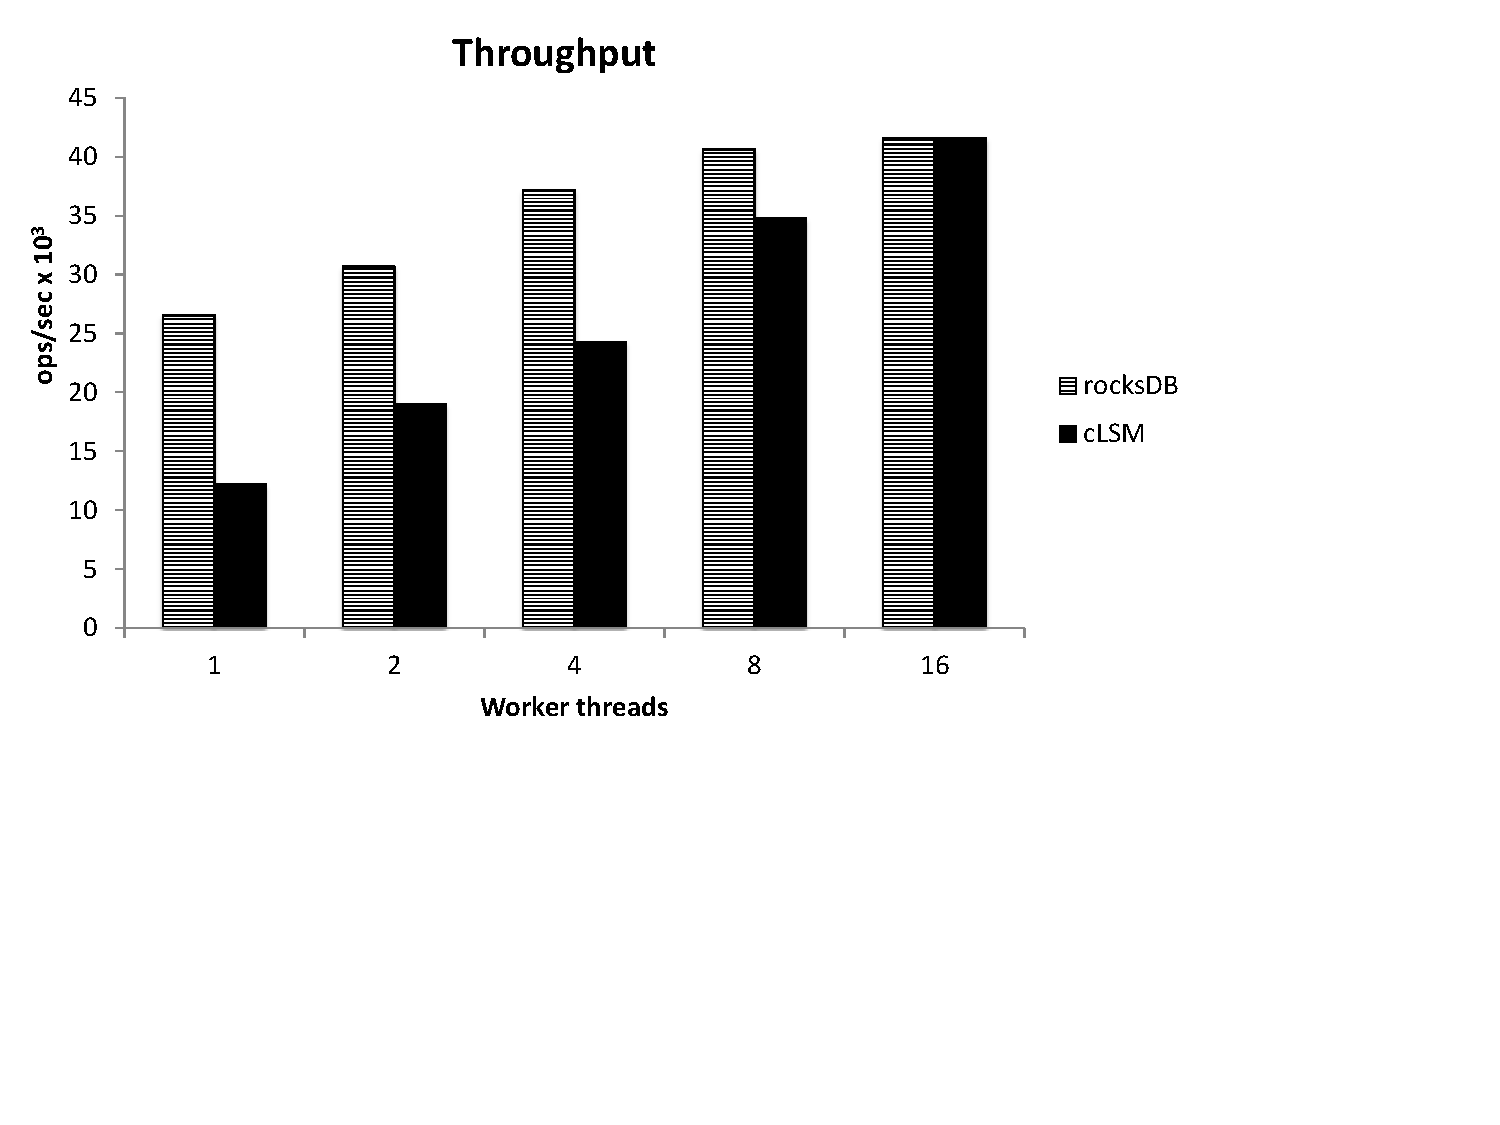
\includegraphics[width=0.45\textwidth,clip, trim =0 180 150 0]{Figures/HeavyCompactions.pdf}}
}
\caption{\bf{Workload with heavy disk-compaction.}}
\label{fig:HeavyCompactions}
\end{figure}
}

Facebook's key-value store, RocksDB~\cite{RocksDB} also builds on {\leveldb}.
%Its memory component supports a single writer and multiple readers.
Much
effort is done in order to reduce critical sections in the memory
component~\cite{RocksDBReduceLocks, RocksDBOptimizedLocks}.
Specifically, readers avoid locks by caching metadata in their thread local storage. Only when a newer
version becomes available readers use locks to get hold of a reference to it.
In addition, the merge process of disk components is executed by multiple
threads concurrently, and some thread is always reserved for flushing the memory
component to the disk.%, thereby avoiding write-stalls.
%RocksDB also supports a basic operator that allows applications to efficiently execute read-modify-write operations.

% bLSM
In the same vein, {\blsm}~\cite{BLSM2012}
introduces a new merge scheduler,
which bounds the time a merge can block write operations.
%In addition, {\blsm}
%leverages Bloom filters~\cite{Bloom1970} to reduce the number of seeks
%(random reads). This results in accelerating searches of items that are not stored in the
%database -- mostly important when invoking an \emph{insert if not
%exists} operation.
As {\blsm} optimizations focus on the merging process and disk
access, it is orthogonal to our work on memory optimizations.



Several approaches for optimizing the performance of the general
logarithmic method have been proposed in recent years.
%
% FD
One such approach suggests adopting a new tree-indexing data structure,
\emph{FD-tree}~\cite{Li2010}, to better facilitate the properties of
contemporary flash disks and solid state drives (SSDs). Like components in LSM-trees, FD-trees maintain multiple
\emph{levels} with cross-level pointers. This approach applies
the \emph{fractional cascading}~\cite{Chazelle86} technique to speed up search
in the logarithmic structure.
%
\remove{
FD-trees aim to (1) minimize the number of
random writes as well as (2) limit them to a small neighborhood, while (3)
preserving high search efficiency. Like the components in LSM-trees, FD-trees
maintain multiple \emph{levels}. Random writes transform into sequential writes
that are initially performed on the top level, and then gradually migrated to
lower levels in batches. The main difference is that instead of having an index
structure at each level (as is the case in LSM components) a level in an
FD-tree holds cross level pointers called \emph{fences} within the sequence of
sorted key entries.
A fence points to a location within the
next level, such that the range between two consecutive fences in level $i$
spans the key range within the page in level $i+1$ that is pointed by the first fence. Essentially,
the cross levels pointers projected by the fences of levels $0\ldots i$ capture
an indexing structure for level $i+1$. Maintaining this implicit structure allows FD-trees
to achieve all 3 properties mentioned above.
}
% FD+
A follow-up work~\cite{FDPlus2012} further refines FD-trees to support
concurrency,  allowing concurrent reads and writes during ongoing index
reorganizations.
\remove{ thus improving both latency and throughput.
The main idea is that a merge of levels $0\ldots m$ progress as a
wavefront within these $m+1$ level. Each level is partitioned into its prefix -- already processed, and yet unprocessed suffix.
The two parts of each level always reflect a single coherent structure. At the
same time, writes are applied to the processed part of the top level, and reads
check the wavefront fence to determine which part of the level to search in.
Blocks in the unprocessed parts are reclaimed only when no new read can go
through them. The top level, which is stored in memory uses a single lock to
control its access. Disk-resident levels use a multi-readers-single-writer lock
per block.
}

With a similar goal of exploiting flash storage as well as the caches of modern
multi-core processors, \emph{Bw-tree}~\cite{LevandoskiLS13} is a new
form of a B-tree, used as an index for a
persistent key-value store.
%To best exploit main memory
The
implementation is non-blocking, allowing for better scalability (throughput). It
also avoids cache line invalidation thus improving cache performance (latency).
Instead of locks, their implementation, which bares similarity to B-link
design~\cite{Lehman1981}, uses CAS instructions, and therefore blocks only
rarely, when fetching a page from disk.
\remove{Attaching delta updates to nodes instead of
performing update-in-place reduces cache invalidation, and thus increases hit
rate.}
At its storage layer, Bw-tree uses log structuring~\cite{RosenblumO1992}.
\remove{It
enables writing large buffers by posting page delta changes, which are
consolidated during a flash cleaning process. Log-structured file system~\cite{RosenblumO1992} is also known to be the source of inspiration
for writing large multi-page blocks to new locations in LSM-trees.
}


%\eshcar{Discuss why our approach is better or explain why we do not compare to
% these solutions. Specifically Bw-tree claims to outperform in-memory
% skip-list.}
None of these new approaches support consistent scans or an atomic RMW
operation (as {\clsm} does). In addition, each of these algorithms builds upon a specific data structure as its
main memory component,
whereas our work can employ any
implementation of a concurrent sorted map to support the basic API.

% % bLSM
% A different approach is presented by {\blsm}~\cite{BLSM2012}. This work
% %improves log structured indexes performance by
% introduces a new merge scheduler,
% which bounds the time a merge can block write operations.
% \remove{The merge process
% ensures that when a component fills, some space becomes available at the next
% component. This significantly reduces the need to block writes to upper levels
% and specifically to $c_0$.
% }
% In addition, {\blsm}
% leverages Bloom filters~\cite{Bloom1970} to reduce the number of seeks
% (random reads). This results in accelerating searches of items that are not stored in the
% database -- mostly important when invoking an \emph{insert if not
% exists} operation.
% \remove{Each disk component is associated with a Bloom filter that
% efficiently represent the items stored in the component with $1\%$ false
% positive rate. This results in each read operation executing $1.03$ seeks in
% expectation, and in accelerating searches of items that are not stored in the
% database. The latter is mostly important when invoking an \emph{insert if not
% exists} operation.
% Bloom filters do not improve scan performance. To address this issue {\blsm}
% choose to bound the number of on-disk components to $3$.
% }
% As {\blsm} optimizations focus on the merging process and disk access, it is
% orthogonal to our work on memory optimizations. We believe the
% two approaches can be combined.

